%\chapterauthor{Author Name}{Author Affiliation}
%\chapterauthor{Second Author}{Second Author Affiliation}
\chapter{Process Management} \label{ch:pm}

A process refers to an instance of a computer program that is running in the system. Managing processes is one of the essential tasks of an OS. In a Windows system, the user can use the task manager, which is a graphical tool to check and manage all the running processes. In a Linux system, the user can manage process in the prompt console using bash commands.

\section{General Introduction to Process}

A process is the fundamental unit for the OS to manage the resources used by a running program.

\subsection{Process}

To improve the efficiency of the CPU, the OS allows multiple processes (also called tasks, jobs) to share the computational capability and memory of the system, each thinking that it is exclusively using the all machine resources, as shown in Fig. \ref{ch:pm:fig:processflow}.

\begin{figure}[htbp]
	\centering
	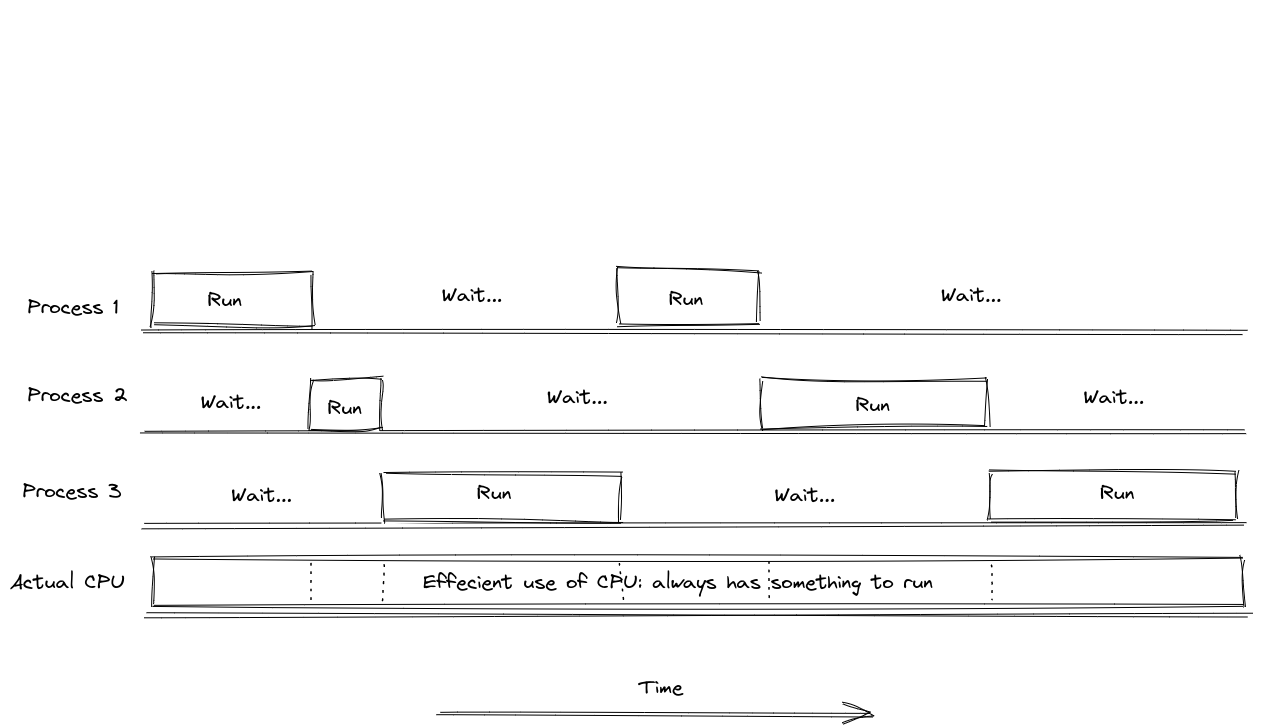
\includegraphics[width=350pt]{chapters/ch-process-management/figures/processflow.png}
	\caption{A demonstration of running multiple processes on a single-core CPU.} \label{ch:pm:fig:processflow}
\end{figure}

The status of a process is stored in its \textit{Process Control Block (PCB)}. The PCB is a special data structure used to describe the dynamic of a process. The OS manages the PCBs and control the processes accordingly. Some of the attributes of a PCB are summarized in Table \ref{ch:pm:tab:pcbcontent}.

\begin{table}
	\centering \caption{Some attributes of a PCB.}\label{ch:pm:tab:pcbcontent}
	\begin{tabularx}{\textwidth}{lX}
		\hline
		Name & Description \\ \hline
		Identifier & The unique ID of the process.  \\ \hdashline
		State & The state of the process, for example, running, suspended, terminated.  \\ \hdashline
		Priority & Priority level in comparison with other processes. \\ \hdashline
		Program Counter & A pointer to the next line of program to be executed. \\ \hdashline
		Memory regions & A pointer to the RAM where the code and data of the process is stored. \\ \hdashline
		Accounting Information & Time limits, clock time used, etc. \\ \hline
	\end{tabularx}
\end{table}

A process shall at least have the following states. The fundamental states of a process and their transferring are introduced in Fig \ref{ch:pm:fig:processstatetransfer}, where ``blocked'' indicates that the process is waiting for other inputs to carry out the remaining part of the program, and ``suspended'' indicates that the process is hold for some reasons. When a process is offloaded from the CPU, its context is moved from the CPU registers to the PCB of the progress.

\begin{figure}[htbp]
	\centering
	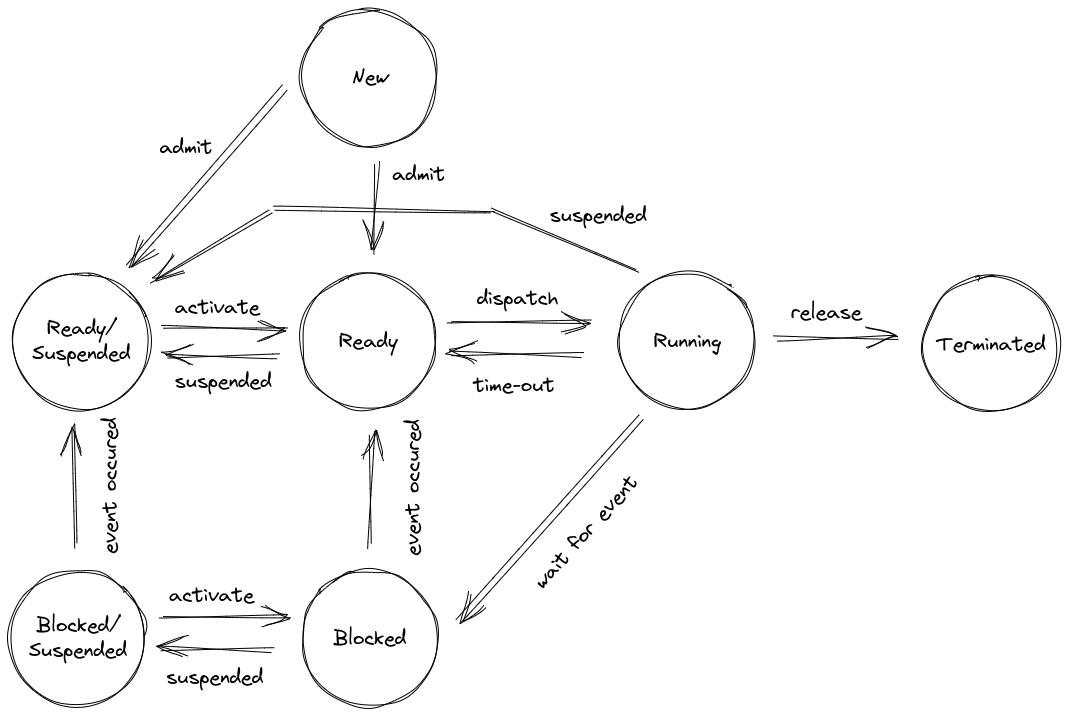
\includegraphics[width=350pt]{chapters/ch-process-management/figures/processstatetransfer.png}
	\caption{Fundamental states of a process and their transferring.} \label{ch:pm:fig:processstatetransfer}
\end{figure}

There are different types of processes. For example, based on the source of the processes, there are OS triggered processes and user triggered processes, the first of which usually has a higher priority. Based on the running environment, there are front-ground processes and background processes. Based on the resources used, there are CPU processes and I/O processes.

A process usually has a relatively isolated environment, and it does not share memory storage with other processes. Special inter process communication mechanism, which is often referred as ``pipe'', is required for processes to talk to each other. Inter process communication requires OS level controls.

\subsection{Thread}

A ``thread'' is like a work dispatch inside a process. There can be multiple threads in a process, as shown in Fig \ref{ch:pm:fig:threadinprocess}. Each thread has its own CPU register values and stack, but they share the same program, memory and file storage addresses.
\begin{figure}[htbp]
	\centering
	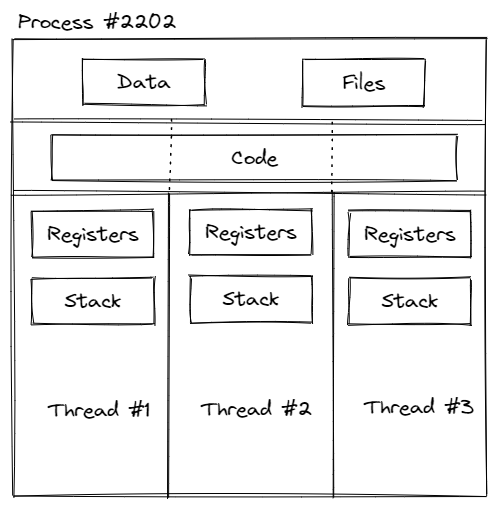
\includegraphics[width=200pt]{chapters/ch-process-management/figures/threadinprocess.png}
	\caption{A demonstration of multiple threads in a process.} \label{ch:pm:fig:threadinprocess}
\end{figure}

Threads differ from processes in the following aspects:
\begin{itemize}
  \item A thread is lighter than a process, occupying less resources to create.
  \item Sharing memories and resources among threads in a process is easier than sharing among processes, because they naturally share address space.
  \item It is easier to enable parallel computation for the threads in the process when it is running on a multi-core CPU.
\end{itemize}

Notice that for many OS, including Linux, the kernel can provide thread level services.

\section{Process Management in Linux}

Two commands, \verb|ps| and \verb|top|, are widely used in monitoring the running process in the OS. They can be used stand-alone, without additional arguments like follows.
\begin{lstlisting}
$ ps
\end{lstlisting}
or
\begin{lstlisting}
$ top
\end{lstlisting}

The major difference between these two commands is that \verb|ps| provides a screenshot (in a text format) of a list of processes including their names, process IDs (PID) and owners, etc., running at the instance, while \verb|top| provides a frequently-refreshing display of the running processes as well as their associated resources usage. Figs \ref{ch:pm:fig:pscommand} and \ref{ch:pm:fig:topcommand} give a quick demo of how the execution of the two commands look like.

\begin{figure}[htbp]
	\centering
	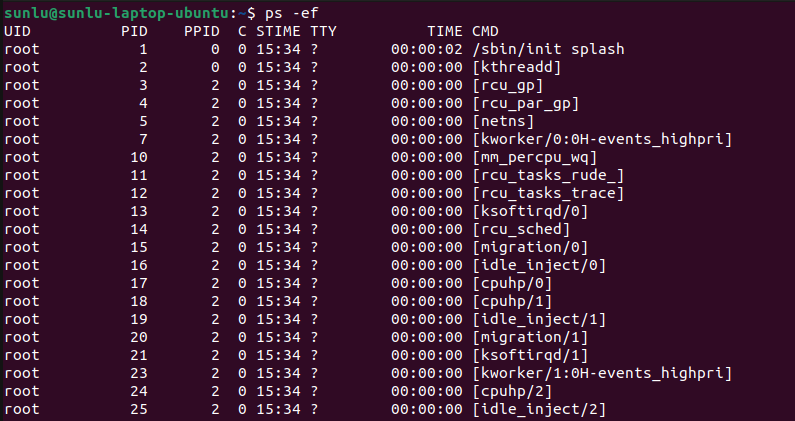
\includegraphics[width=300pt]{chapters/ch-process-management/figures/pscommand.png}
	\caption{Execution of \texttt{ps} command.} \label{ch:pm:fig:pscommand}
\end{figure}

\begin{figure}[htbp]
	\centering
	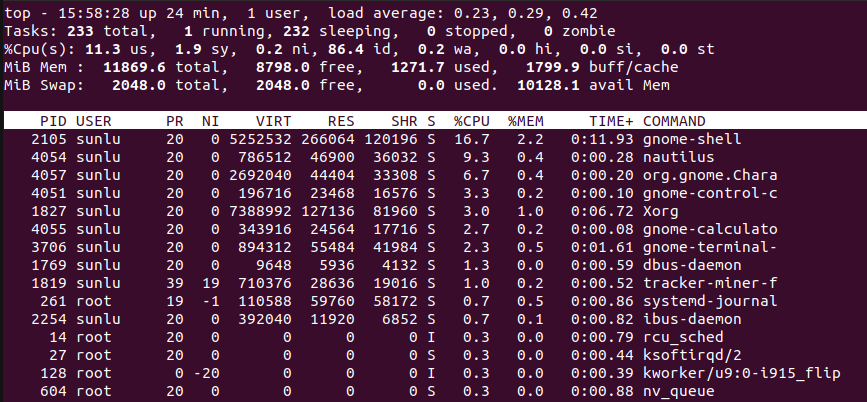
\includegraphics[width=300pt]{chapters/ch-process-management/figures/topcommand.png}
	\caption{Execution of \texttt{top} command.} \label{ch:pm:fig:topcommand}
\end{figure}

Notice that \verb|top| is a running application where the user can keep interacting with to filter for particular processes, while \verb|ps| is more of a one-time command and its output can be saved into a text file for further processing.

To kill a process, use the \verb|kill| command as follows.
\begin{lstlisting}
$ kill <option> <process ID>
\end{lstlisting}

The \verb|kill| command offers different options to kill a process. Use \verb|kill -l| to list down the options as given below (and many more).
\begin{lstlisting}
1) SIGHUP    2) SIGINT    3) SIGQUIT   4) SIGILL
5) SIGTRAP   6) SIGABRT   7) SIGBUS    8) SIGFPE
9) SIGKILL  10) SIGUSR1  11) SIGSEGV  12) SIGUSR2
13) SIGPIPE 14) SIGALRM	 15) SIGTERM  16) SIGSTKFLT
17) SIGCHLD 18) SIGCONT	 19) SIGSTOP  20) SIGTSTP
...
\end{lstlisting}

Commonly used \verb|kill| options are \verb|kill -9| and \verb|kill -15| followed by the PID. Notice that in Linux the process is arranged in a tree structure; killing a parent process will automatically terminate its children processes, and killing a child process may result in its parent process to restart a new child process.
